
% Copyright 2020 by Robert Hildebrand
%This work is licensed under a
%Creative Commons Attribution-ShareAlike 4.0 International License (CC BY-SA 4.0)
%See http://creativecommons.org/licenses/by-sa/4.0/

%\documentclass[../open-optimization/open-optimization.tex]{subfiles}
%
%\begin{document}

\chapter{Mathematical Programming}
\todoChapter{ 50\% complete. Goal 80\% completion date: August 20\\
Notes: This chapter is meant to be an introduction to all the types of deterministic problems that we might discuss.  It should list many applications, have a number of pictures, and describe how and where these types of problems are used.  }

\todo[inline]{Add intro that explains the format of problems, i.e., what the complexity comment means in each problem and add pointer to section on computational complexity.}
\todo[inline]{
Add discussion of Optimization, Operations Research, and Mathematical Programming including background and applications.   
Also, give an introduction to the content in this book, what you will learn by working though the book, and why this book is interesting and different from other sources.}



We will state main general problem classes to be associated with in these notes.  These are Linear Programming (LP), Mixed-Integer Linear Programming (MILP), Non-Linear Programming (NLP), and Mixed-Integer Non-Linear Programming (MINLP).  


%\begin{center}
%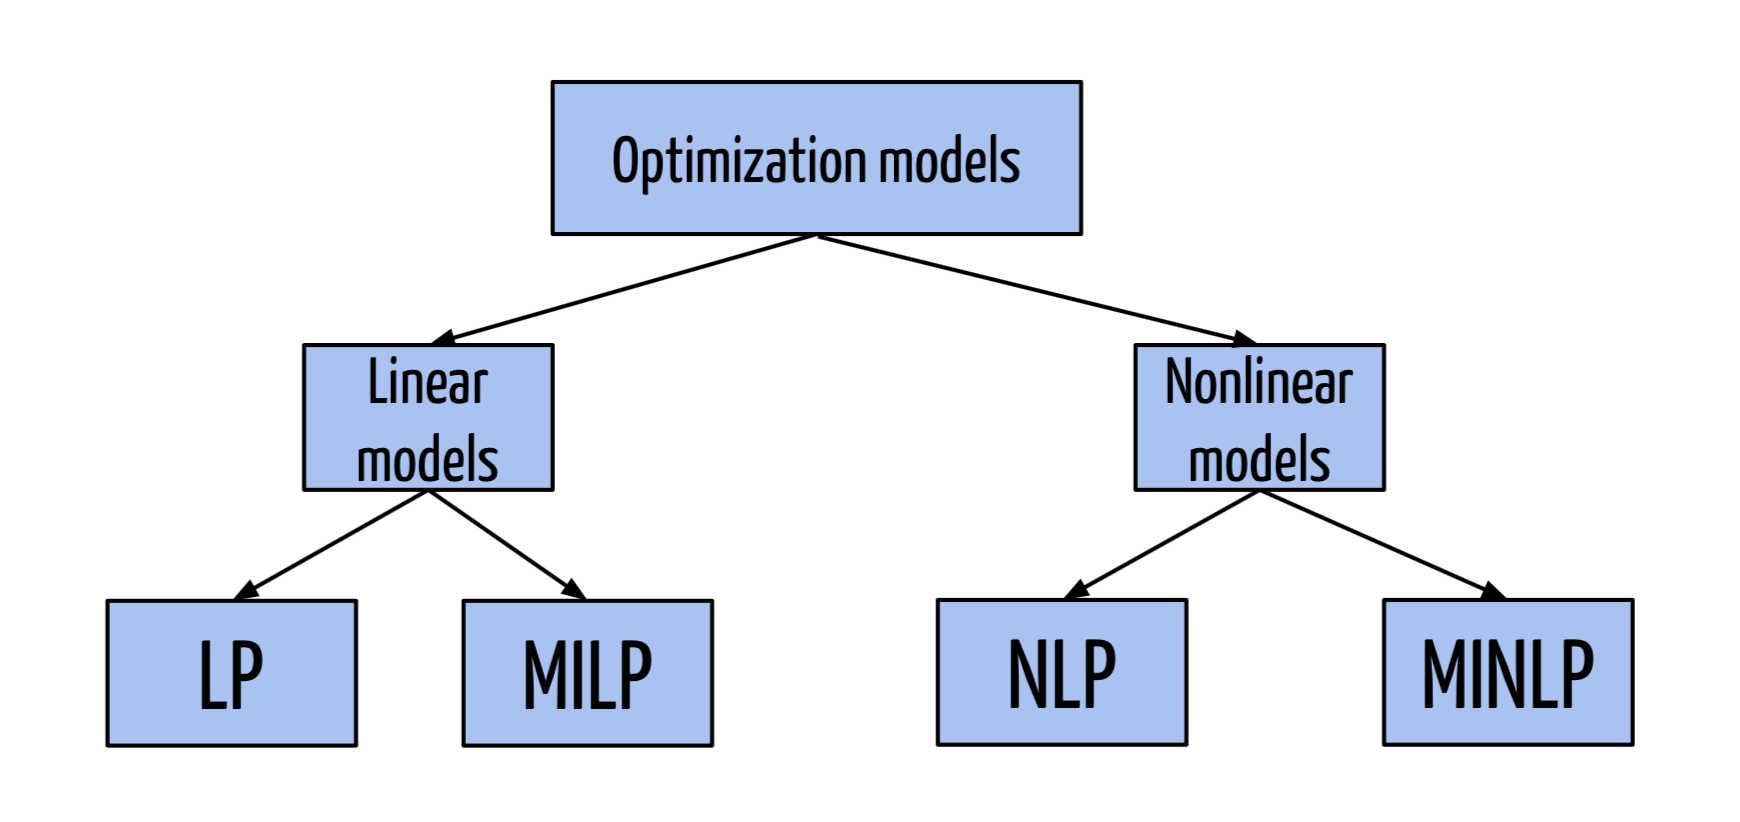
\includegraphics[scale = 0.5]{problem-class-diagram}\footnote{Diagram by Diego Moran}
%\end{center}

\includefigurestatic[][width = 1\linewidth][h]{problem-class-diagram}

Along with each problem class, we will associate a complexity class for the general version of the problem.  See \autoref{sec:complexity} for a discussion of complexity classes.  Although we will often state that input data for a problem comes from $\R$, when we discuss complexity of such a problem, we actually mean that the data is rational, i.e., from $\Q$, and is given in binary encoding.

\section{Linear Programming (LP)}
\todo[inline]{Describe applications and andd images}
Some linear programming background, theory, and examples will be provided in \autoref{sec:LP-background}.
\begin{general}{Linear Programming (LP)}{\polynomial}
%\label{general:LP}
Given a matrix $A \in \R^{m\times n}$, vector $b \in \R^m$ and vector $c \in \R^n$, the \emph{linear programming} problem is
\begin{equation}
\label{eq:LP}
\begin{split}
\max \quad & c^\top x\\
\st  \quad & Ax \leq b\\
& x \geq 0
\end{split}
\end{equation}
\end{general}

Linear programming can come in several forms, whether we are maximizing or minimizing, or if the constraints are $\leq, =$ or $\geq$.   One form commonly used is \emph{Standard Form} given as 
\begin{general}{Linear Programming (LP) Standard Form}{\polynomial}
Given a matrix $A \in \R^{m\times n}$, vector $b \in \R^m$ and vector $c \in \R^n$, the \emph{linear programming} problem in \emph{standard form} is
\begin{equation}
\label{eq:standardLP}
\begin{split}
\max \quad & c^\top x\\
\st  \quad & Ax = b\\
& x \geq 0
\end{split}
\end{equation}
\end{general}

\refincludefigurestatic[Linear programming constraints and objective.][scale = 0.2][h]{wiki/File/linear-programming.png}


\begin{exercise}
\label{exercise:LPconversion}
Start with a problem in form given as \eqref{eq:LP} and convert it to standard form \eqref{eq:standardLP} by adding at most $m$ many new variables and by enlarging the constraint matrix $A$ by at most $m$ new columns.
\end{exercise}
\section{Mixed-Integer Linear Programming (MILP)}
Mixed-integer linear programming will be the focus of Sections \ref{sec:IP-formulations},\ref{sec:exponential-IP-forumulations}, \ref{sec:IP-algorithms}, and \ref{sec:IP-heuristics}.
Recall that the notation $\Z$ means the set of integers and the set $\R$ means the set of real numbers.  The first problem of interest here is a \emph{binary integer program} (BIP) where all $n$ variables are binary (either 0 or 1).

\begin{general}{Binary Integer programming (BIP)}{\npcomplete}
Given a matrix $A \in \R^{m\times n}$, vector $b \in \R^m$ and vector $c \in \R^n$, the \emph{binary integer programming} problem is
\begin{equation}
\label{eq:BIP}
\begin{split}
\max \quad & c^\top x\\
\st  \quad & Ax \leq b\\
& x \in \{0,1\}^n
\end{split}
\end{equation}
\end{general}
A slightly more general class is the class of \emph{Integer Linear Programs} (ILP).  Often this is referred to as \emph{Integer Program} (IP), although this term could leave open the possibility of non-linear parts.

\refincludefigurestatic[Comparing the LP relaxation to the IP solutions.][scale = 0.3][h]{wiki/File/integer-programming.png}


\begin{general}{Integer Linear Programming (ILP)}{\npcomplete}
Given a matrix $A \in \R^{m\times n}$, vector $b \in \R^m$ and vector $c \in \R^n$, the \emph{integer linear programming} problem is
\begin{equation}
\label{eq:ILP}
\begin{split}
\max \quad & c^\top x\\
\st  \quad & Ax \leq b\\
& x \in \Z^n
\end{split}
\end{equation}
\end{general}


An even more general class is \emph{Mixed-Integer Linear Programming (MILP)}.  This is where we have $n$ integer variables $x_1, \dots, x_n \in \Z$ and $d$ continuous variables $x_{n+1}, \dots, x_{n+d} \in \R$.  Succinctly, we can write this as $x \in \Z^n \times \R^d$, where $\times$ stands for the \emph{cross-product} between two spaces.   

Below, the matrix $A$ now has $n+d$ columns, that is, $A \in \R^{m \times n+d}$.  Also note that we have not explicitly enforced non-negativity on the variables.  If there are non-negativity restrictions, this can be assumed to be a part of the inequality description $Ax \leq b$.
\begin{general}{Mixed-Integer Linear Programming (MILP)}{\npcomplete}
Given a matrix $A \in \R^{m\times (n+d)}$, vector $b \in \R^m$ and vector $c \in \R^{n+d}$, the \emph{mixed-integer linear programming} problem is
\begin{equation}
\label{eq:ILP}
\begin{split}
\max \quad & c^\top x\\
\st  \quad & Ax \leq b\\
& x \in \Z^n \times \R^d
\end{split}
\end{equation}
\end{general}

\section{Non-Linear Programming (NLP)}
\begin{general}{NLP}{\nphard}
Given a function $f(x)\colon \R^d \to \R$ and other functions $f_i(x)\colon \R^d \to \R$ for $i=1, \dots, m$,  the \emph{nonlinear programming} problem is
\begin{equation}
\label{eq:convex-programming}
\begin{split}
\min \quad & f(x)\\
\st  \quad & f_i(x) \leq 0  \quad  \text{ for } i=1, \dots, m\\
& x \in \R^d
\end{split}
\end{equation}
\end{general}


Nonlinear programming can be separated into convex programming and non-convex programming.  These two are very different beasts and it is important to distinguish between the two.
\subsection{Convex Programming}
Here the functions are all \textbf{convex!}
\begin{general}{Convex Programming}{\polynomial\ \  (typically)}
Given a convex function $f(x)\colon \R^d \to \R$ and convex functions $f_i(x)\colon \R^d \to \R$ for $i=1, \dots, m$,  the \emph{convex programming} problem is
\begin{equation}
\label{eq:convex-programming}
\begin{split}
\min \quad & f(x)\\
\st  \quad & f_i(x) \leq 0  \quad  \text{ for } i=1, \dots, m\\
& x \in \R^d
\end{split}
\end{equation}
\end{general}
\begin{example}{}{}
Convex programming is a generalization of linear programming.  This can be seen by letting $f(x) = c^\top x$ and $f_i(x) = A_i x - b_i$.  
\end{example}
\subsection{Non-Convex Non-linear Programming}
When the function $f$ or functions $f_i$ are non-convex, this becomes a non-convex nonlinear programming problem.  There are a few complexity issues with this.

\paragraph{IP as NLP}
As seen above, quadratic constraints can be used to create a feasible region with discrete solutions.  For example 
$$
x(1-x) = 0
$$
has exactly two solutions: $x = 0, x=1$.  
Thus, quadratic constraints can be used to model binary constraints.
\begin{general}{Binary Integer programming (BIP) as a NLP}{\nphard}
Given a matrix $A \in \R^{m\times n}$, vector $b \in \R^m$ and vector $c \in \R^n$, the \emph{binary integer programming} problem is
\begin{equation}
\label{eq:BIP}
\begin{split}
\max \quad & c^\top x\\
\st  \quad & Ax \leq b\\
& \hcancel[1.5pt]{x \in \{0,1\}^n}\\
& x_i(1-x_i) = 0 \quad \text{ for } i=1, \dots, n
\end{split}
\end{equation}
\end{general}
\subsection{Machine Learning}
\todo[inline]{Many machine learning problems fall into this catrgory.  Todo: describe applications, give references, etc.}
\section{Mixed-Integer Non-Linear Programming (MINLP)}
\todo[inline]{Fill in this section with formulas and discuss applications.  Most notable applications are Electrical Grid problems and Pooling problems. Find applications at Optimization and Engineering \url{https://link.springer.com/journal/11081/volumes-and-issues/21-4}}
\subsection{Convex Mixed-Integer Non-Linear Programming}

\subsection{Non-Convex Mixed-Integer Non-Linear Programming}





%
%
%\end{document}
